\question 流水线计算机中,下列语句发生的数据相关类型是 ADD R1,R2,R3;(R2)+(R3)→R1
ADD R4,R1,R5;(R1)+(R5)→R4
\par\twoch{写后写}{读后写}{\textcolor{red}{写后读}}{读后读}
\begin{solution}C。
数据相关包括RAW(写后读)、WAW(写后写)、WAR(读后写)。设有i和j两条指令,i指令在前,j指令在后,则3种相关的含义如下。
●RAW(写后读):指令j试图在指令i写入寄存器前就读出该寄存器的内容,这样指令j就会错误地读出该寄存器旧的内容。
●WAR(读后写):指令j试图在指令i读出该寄存器前就写入该寄存器,这样指令i就会错误地读出该寄存器的新内容。
●WAW(写后写):指令j试图在指令i写入寄存器前就写入该寄存器,这样两次写的先后次序被颠倒,就会错误地使由指令i写入的值成为该寄存器的内容。
在这两条指令中,都对R1进行操作,其中前面对R1写操作,后面对R1读操作,因此发生写后读相关。
\end{solution}
\question 在指令流水线中为解决数据相关经常使用的方法有( )。 I.插入nop指令
II.猜测法 III.改变指令执行顺序 IV.设置相关的数据通路
\par\twoch{I和III}{II和IV}{I、II和III}{\textcolor{red}{I、III和IV}}
\begin{solution}NOP是英语No
Operation的缩写。NOP无操作数,所以称为空操作。执行NOP指令只使程序计数器PC加1,所以占用一个机器周期。插入NOP指令的方法,在发生数据相关冲突的指令之间插入空操作指令能避免数据冲突,故I是。
猜测法是解决控制相关使用的方法,故II不是。
当发现上下两条指令数据相关的时候,可以不中止流水线,而通过优化编译器将下一条指令之后不产生相关的指令提前执行,从而避免数据冲突,故III是。
在运算部件中设置一些数据寄存区及专用通路,使前条指令的运算结果通过专用通道直接送入后续的运算部件,故IV是。
综上,本题选D。
\end{solution}
\question 以下关于结构相关冲突的叙述错误的是
\par\fourch{结构相关冲突是指同时有多条指令使用同一资源}{\textcolor{red}{避免结构相关冲突的基本做法是使每个指令在相同的流水段中使用不同的功能部件}}{重复设置功能部件可以避免结构相关冲突}{数据Cache和指令Cache分离可解决同时访问数据和指令的冲突}
\begin{solution}如下图中,每个指令的五个流水段分别对应五个独立的功能部件。这时指令I4的IF流水段,如果跟I1的IF流水段使用相同的功能部件,那么它就不会和I1指令的MEM流水段发生结构相关冲突。故避免结构相关冲突的基本做法是使每个指令在相同的流水段中使用相同的功能部件。故B为错误的选项。
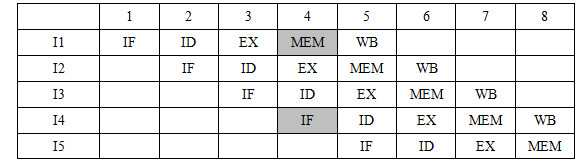
\includegraphics[width=6.06250in,height=1.71875in]{computerassets/fa5c1b2b874ee2b1d0efe52dadf7e098.png}
其他选项都为正确的叙述。
\end{solution}
\question 以下关于数据相关冲突的叙述中正确的有( )。
I.数据相关冲突指的是流水线中的各条指令因重叠操作,可能改变对操作数的读写访问顺序。
II.在发生数据相关冲突的指令之间插入空操作指令能避免数据冲突
III.采用旁路技术可以解决部分数据相关冲突
IV.通过编译器调整指令顺序可解决部分数据相关冲突
\par\twoch{I和III}{I、II和III}{II和III}{\textcolor{red}{全部}}
\begin{solution}I选项是对数据相关冲突的正确定义,故I正确。
II、III和IV都是是解决数据相关冲突的方法,故也都是正确的,故本题应该选D。
\end{solution}
\question 以下关于控制相关冲突的叙述中,错误的是
\par\fourch{条件转移指令执行时可能会发生控制相关冲突}{在分支指令后加入若干空操作指令可避免控制相关冲突}{\textcolor{red}{采用数据旁路技术可以解决部分控制相关冲突}}{通过编译器调整指令顺序可解决部分控制相关冲突}
\begin{solution}其中A、B、D都是正确的描述。
数据旁路技术只能解决数据相关冲突,跟控制相关冲突完全无关,故C选项错误。
【总结】
通过加空操作,可以解决结构相关冲突、数据相关冲突和控制相关冲突,为什么呢?通过加空操作,其实就是牺牲了流水线的``并行性'',在极端情况下,即加的空指令够多的情况下,会恢复到无流水线的情况。因此,通过加空操作,可以解决全部的冲突。
通过编译器调整指令顺序,可``部分''解决这三类冲突。若出现这类描述也是正确的。
\end{solution}
\question 下面是一段MIPS指令序列:
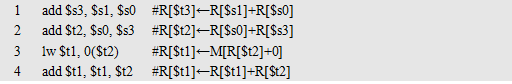
\includegraphics[width=5.33333in,height=0.87500in]{computerassets/e3e987b0dc6aa40b5c4452ae4b71aef8.png}

以上指令序列中,哪些指令之间发生数据相关?
\par\fourch{1和2、2和3}{1和2、2和4}{1和3、2和3、2和4、3和4}{\textcolor{red}{1和2、2和3、2和4、3和4}}
\begin{solution}第1条和第2条指令之间关于\$s3数据相关。
第2条和第3条指令之间关于\$t2数据相关。
第2条和第4条指令之间关于\$t2数据相关。
第3条和第4条指令之间关于\$t1数据相关。 故本题选D。
\end{solution}
\question 某CPU主频为1.03GHz,采用4级指令流水线,每个流水段的执行需要1个时钟周期。假定CPU执行了100条指令,在其执行过程中,没有发生任何流水线阻塞,此时流水线的吞吐率为(
)
\par\fourch{$0.25×10^9$条指令/秒}{$0.97×10^9$条指令/秒}{\textcolor{red}{$1.0×10^9$条指令/秒}}{$1.03×10^9$条指令/秒}
\begin{solution}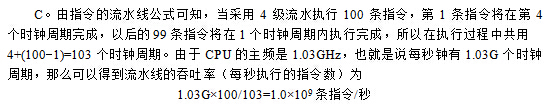
\includegraphics[width=5.73958in,height=1.09375in]{computerassets/7e707ae279824ceb7945f57d5c919616.jpeg}
\end{solution}
